


\documentclass[a4paper,12pt]{article}

\usepackage{cmap}					% поиск в PDF
\usepackage[T2A]{fontenc}			% кодировка
\usepackage[utf8]{inputenc}			% кодировка исходного текста
\usepackage[english,russian]{babel}	% локализация и переносы
\usepackage[left=2cm,right=2cm,top=2cm,bottom=2cm,bindingoffset=0cm]{geometry}
\usepackage{graphicx}
\usepackage{float}%"Плавающие" картинки
\usepackage{wrapfig}%Обтекание фигур (таблиц, картинок и прочего)
\usepackage{parskip}
\usepackage{mathtext}

\setlength{\parindent}{2em}
\setlength{\parskip}{2em}


\author{Имя Автора}
\title{1.1 Наш первый документ}
\date{\today}

\begin{document} % Конец преамбулы, начало текста.
\center
\newcommand{\HRule}{\rule{\linewidth}{0.3 mm}} % Defines a Hnew command for the horizontal lines, change thickness here
\textsc{\Large Київський національний університет ім.Т.Шевченка }\\[1.5cm] % Name of your university/college
\textsc{\Large Фізичний факультет}\\[2.5cm] % Major heading such as course name

%----------------------------------------------------------------------------------------
%	TITLE SECTION
%----------------------------------------------------------------------------------------

\HRule \\[0.4cm]
{ \huge \bfseries Моделювання ВАХ діодів}\\[0.4cm] % Title of your document
\HRule \\[1.5cm]

%----------------------------------------------------------------------------------------
%	AUTHOR SECTION
%----------------------------------------------------------------------------------------
\flushright
\begin{minipage}{0.4\textwidth}
\large
\emph{Автор:}\\ Холоімов Валерій % Your name
\end{minipage}\\[15cm]
\center
%	DATE SECTION
%----------------------------------------------------------------------------------------

{\large \today}\\[2cm] % Date, change the \today to a set date if you want to be precise
\flushleft




\tableofcontents

\newpage

\section{Вступна частина}
\subsection{Об'єкт дослідження}
Визначення вольт-амперної характеристики діодів. Моделюванння ВАХ діодів.
\subsection{Мета}
Дослідити ВАХ діодів. Порівняти ВАХ різних діодів.
\subsection{Методи дослідження}
Один з каналів отримує напругу на діоді. Другий канал отримує напругу на відомому резисторі, що дає можливість визначити нам сили струму на ділянці кола. На екрані двоканального осцилографа спостерігаємо графік залежності напруги на діоді від сили струми на ділянці колі.

\section{Теоретична частина}
\subsection{Термінологія}


\qquad \textbf{Діод}  Електроний прилад, що пропускає струм лише в одном напрямку. Має відміну від провідника у власній будові, тому ВАХ діода має певну відмінність від ВАХ резистора. \par
\textbf{Осцилограф} Прилад, що призначений для вимірювання, спостерігання та запису параметрів електричного сигналу. У роботі використовуємо осцилограф для побудови залежності напргуи на діоді від сили струму на ділянці кола. \par
\textbf{Резистор}  пасивний елемент електричного кола, призначений для використання його електричного опору. Основною характеристикою резистора є величина його електричного опору. Для випадку лінійної характеристики, значення електричного струму крізь резистор в залежності від електричної напруги, описується законом Ома.

\newpage


\section{Практична частина}
\subsection{Вступ до практичної частини}
\qquad	 В методичці "Вивчення радіоелектронних схем методом комп'ютерного моделювання" можна знайти схему, що допомагає нам отримати значення сили струму на ділянці кола і напругу на діоді. Для складання цієї схеми нам необхідно використати наступні компоненти: \par
\indent \hspace{1em} резистор опором 10 Ом, \newline
\indent \hspace{1em} діоди BH01Pasd, \newline
\indent \hspace{1em} XSC1 - осцилогаф,\newline
\indent \hspace{1em} XFG1 - функціональний генератор,\newline
\indent \hspace{1em} ключі K1, K2, K3.\par
Переключаючи ключі, можемо отримати ВАХ для кожного з діодів а також їх комбінацій.
\begin{figure}[ht]

\centering

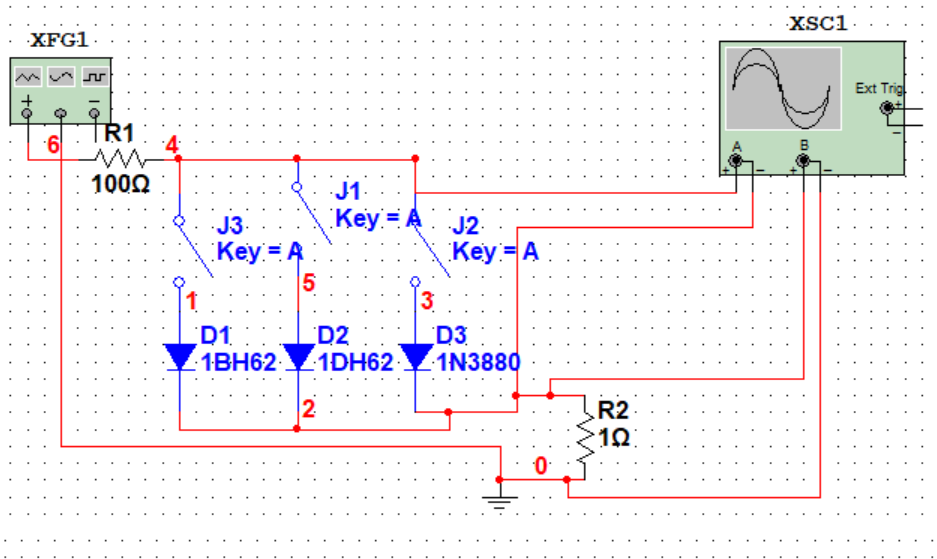
\includegraphics[width=0.8\linewidth]{Схема.png}

\caption{CСхема, що використовувалась у роботі}

\label{fig:mpr}

\end{figure}

\newpage
\subsection{Діод 1}
\begin{figure}[ht]

\centering

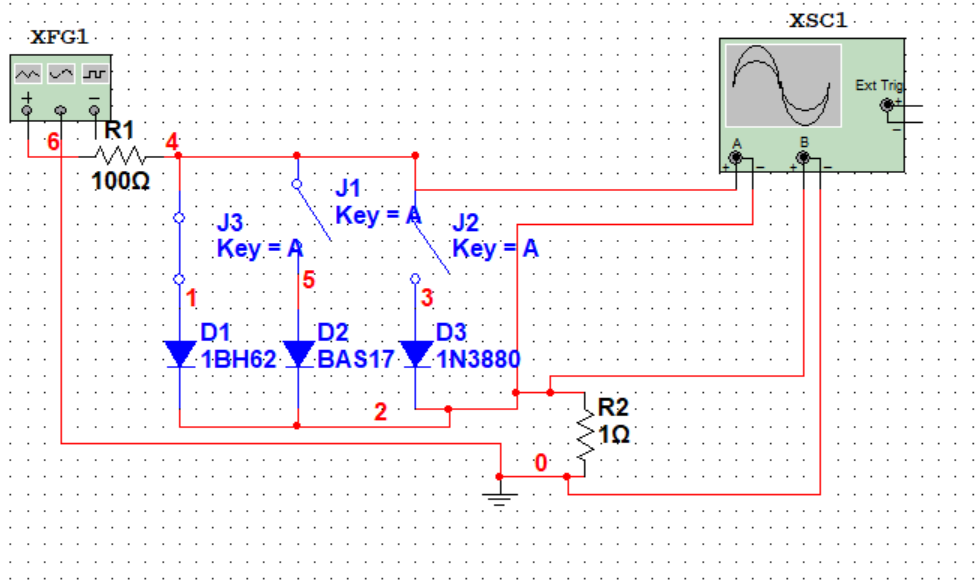
\includegraphics[width=0.6\linewidth]{Діод1Схема.png}

\caption{Схема}

\label{Diod1Shema}

\end{figure}

\begin{figure}[ht]

\centering

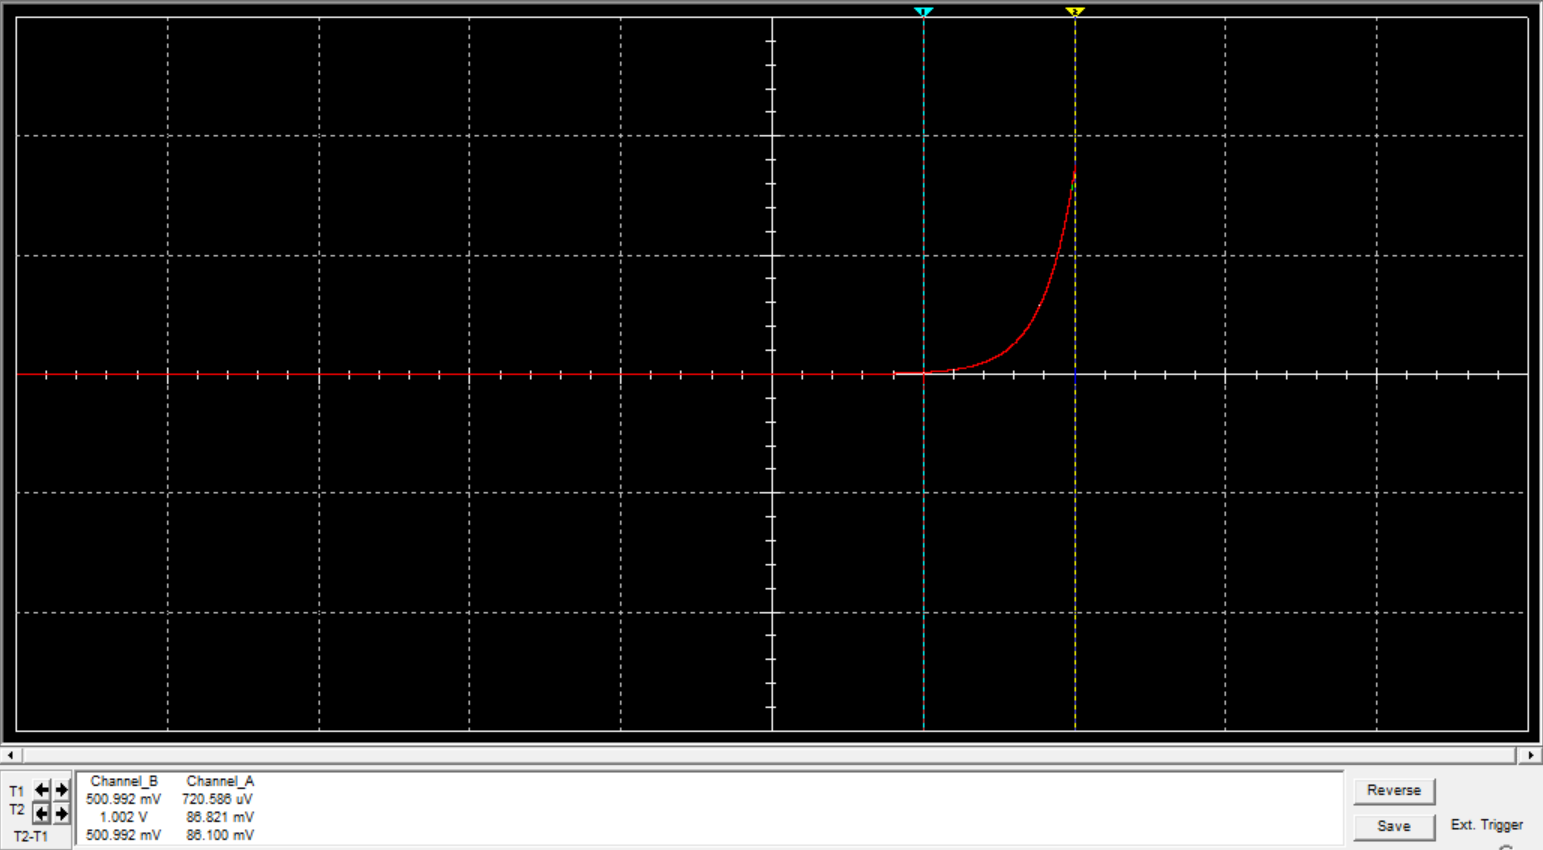
\includegraphics[width=0.75\linewidth]{Діод1Осцилограф.png}

\caption{Результати вимірів}

\label{Diod1Osc}

\end{figure}

\begin{figure}[ht]

\centering

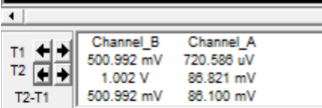
\includegraphics[width=0.3\linewidth]{Діод1Рез.png}

\caption{Результати вимірів}

\label{Diod1Rez}

\end{figure}

Оскільки канал А виводить напругу на резисторі опором $1  \Omega $, можемо вважати, що отримані значення - сила струму у колі.

\newpage
\subsection{Діод 2}
\begin{figure}[ht]

\centering

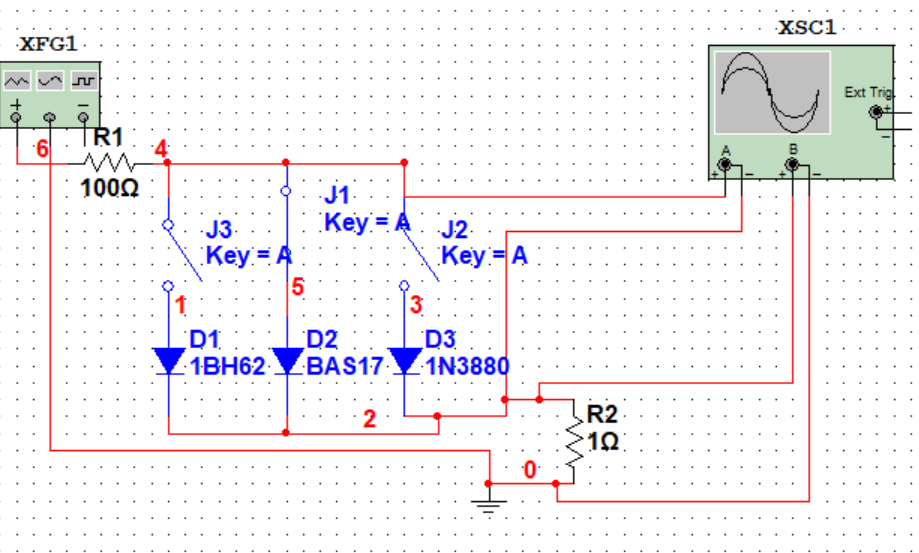
\includegraphics[width=0.6\linewidth]{Діод2Схема.png}

\caption{Схема}

\label{Diod2Shema}

\end{figure}

\begin{figure}[ht]

\centering

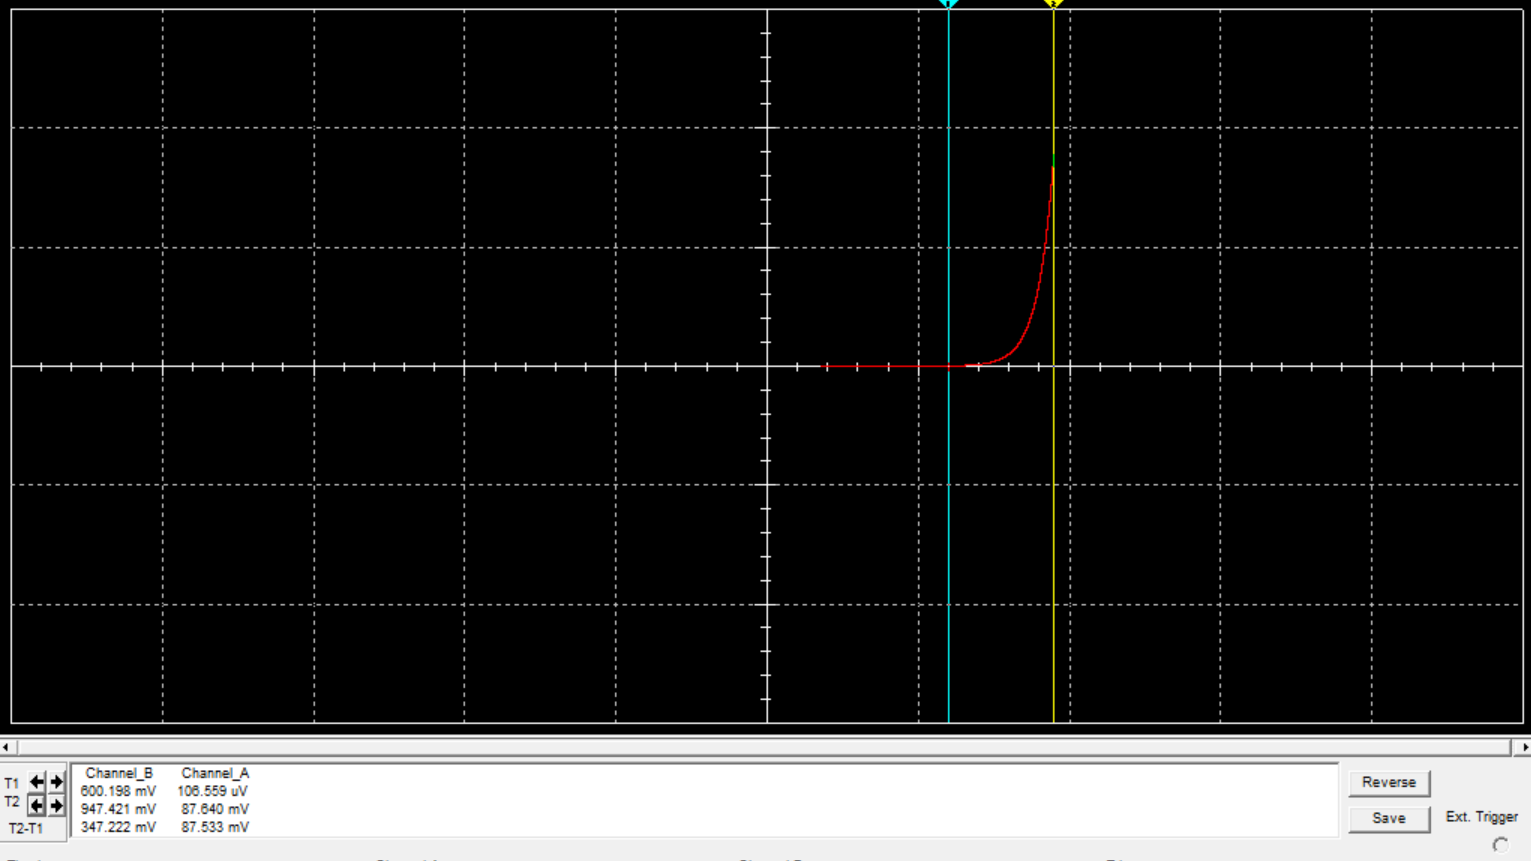
\includegraphics[width=0.75\linewidth]{Діод2Осцилограф.png}

\caption{Результати вимірів}

\label{Diod2Osc}

\end{figure}

\begin{figure}[ht]

\centering

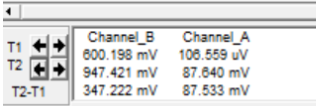
\includegraphics[width=0.3\linewidth]{Діод2Рез.png}

\caption{Результати вимірів}

\label{Diod2Rez}

\end{figure}

\newpage
\subsection{Діод 3}
\begin{figure}[ht]

\centering

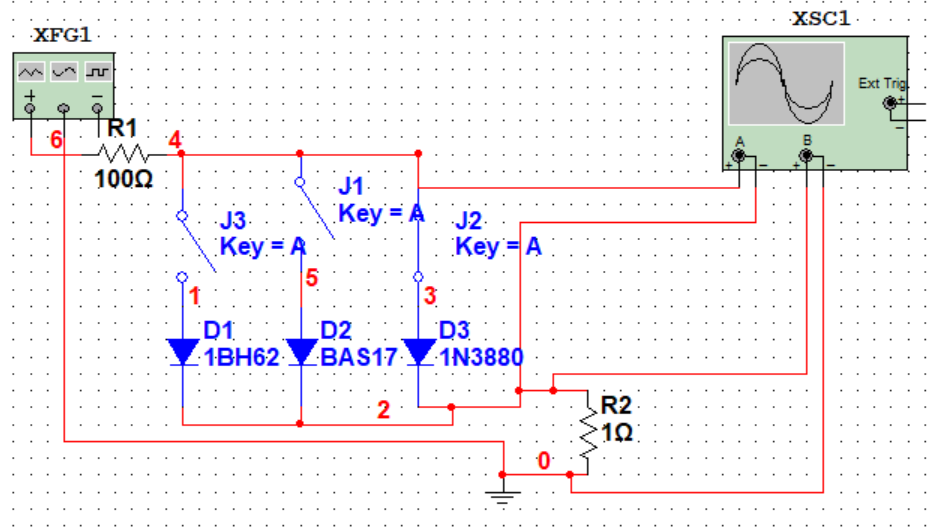
\includegraphics[width=0.6\linewidth]{Діод3Схема.png}

\caption{Схема}

\label{Diod3Shema}

\end{figure}

\begin{figure}[ht]

\centering

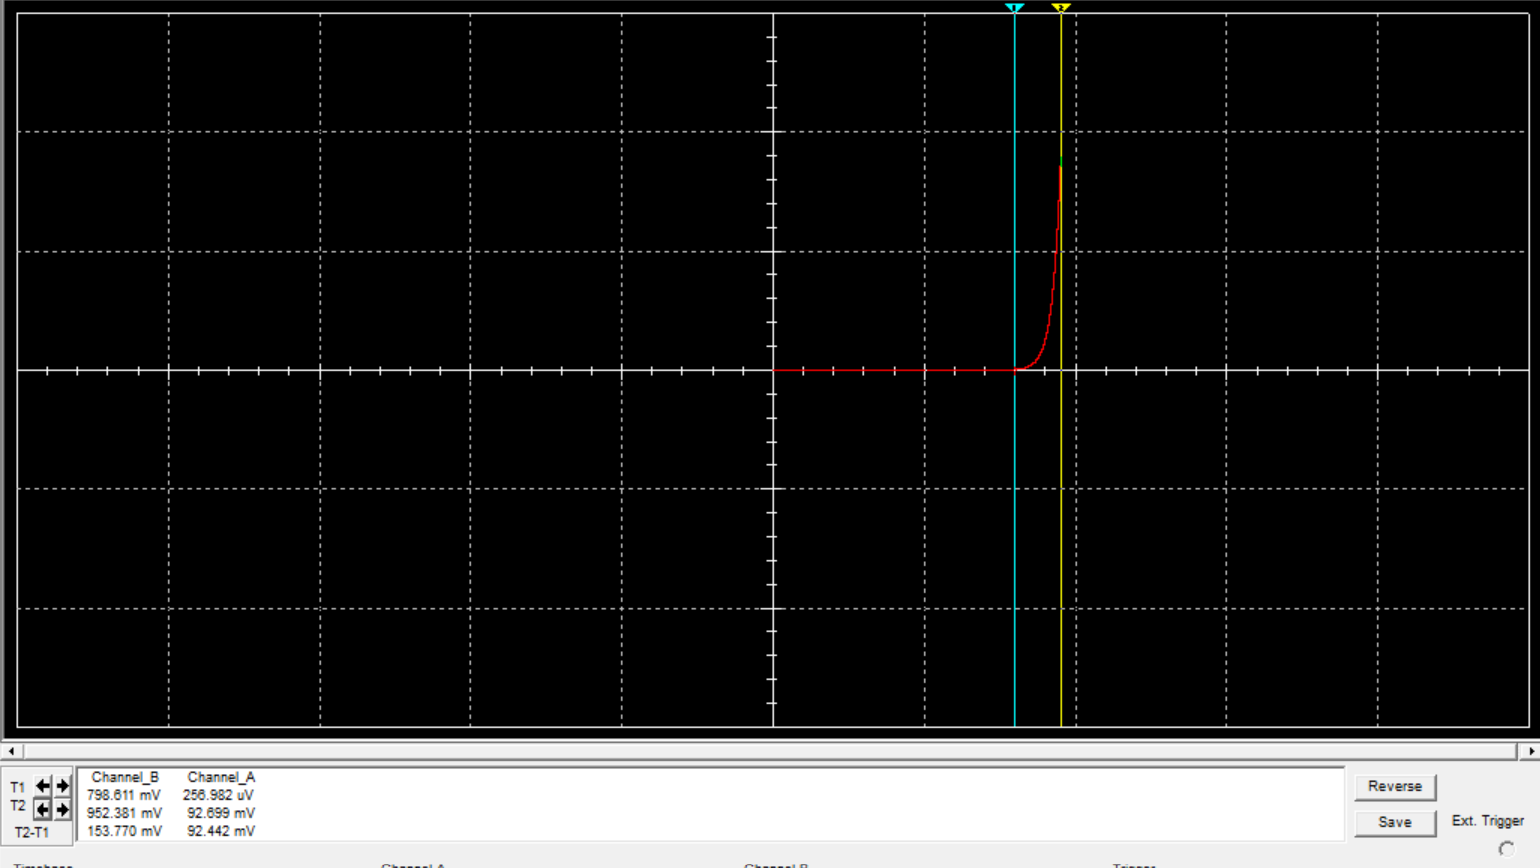
\includegraphics[width=0.75\linewidth]{Діод3Осцилограф.png}

\caption{Результати вимірів}

\label{Diod3Osc}

\end{figure}

\begin{figure}[ht]

\centering

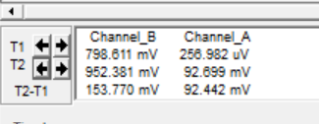
\includegraphics[width=0.3\linewidth]{Діод3Рез.png}

\caption{Результати вимірів}

\label{Diod3Rez}

\end{figure}

\newpage
\subsection{Робота з Arduino}
\input{Ардуино}






\section{Відповіді на контрольні запитання}
\subsection{Контрольне питання 1}











\end{document} % Конец текста.
